% Renders the report's three figures as standalone pages for the README images.
% Build: pdflatex figs_standalone.tex  ->  three-page PDF, one figure per page.
\documentclass[tikz,border=10pt]{standalone}
\usepackage[T1]{fontenc}
\usepackage{lmodern}
\usepackage{amsmath}
\usepackage{xcolor}
\definecolor{acc}{RGB}{31,71,136}
\definecolor{accB}{RGB}{40,105,95}
\definecolor{meas}{RGB}{176,124,34}
\usetikzlibrary{positioning,arrows.meta,fit,calc,backgrounds}
\usepackage{pgfplots}
\pgfplotsset{compat=1.17}
\begin{document}

% ---------------------------------------------------------------- figure 1
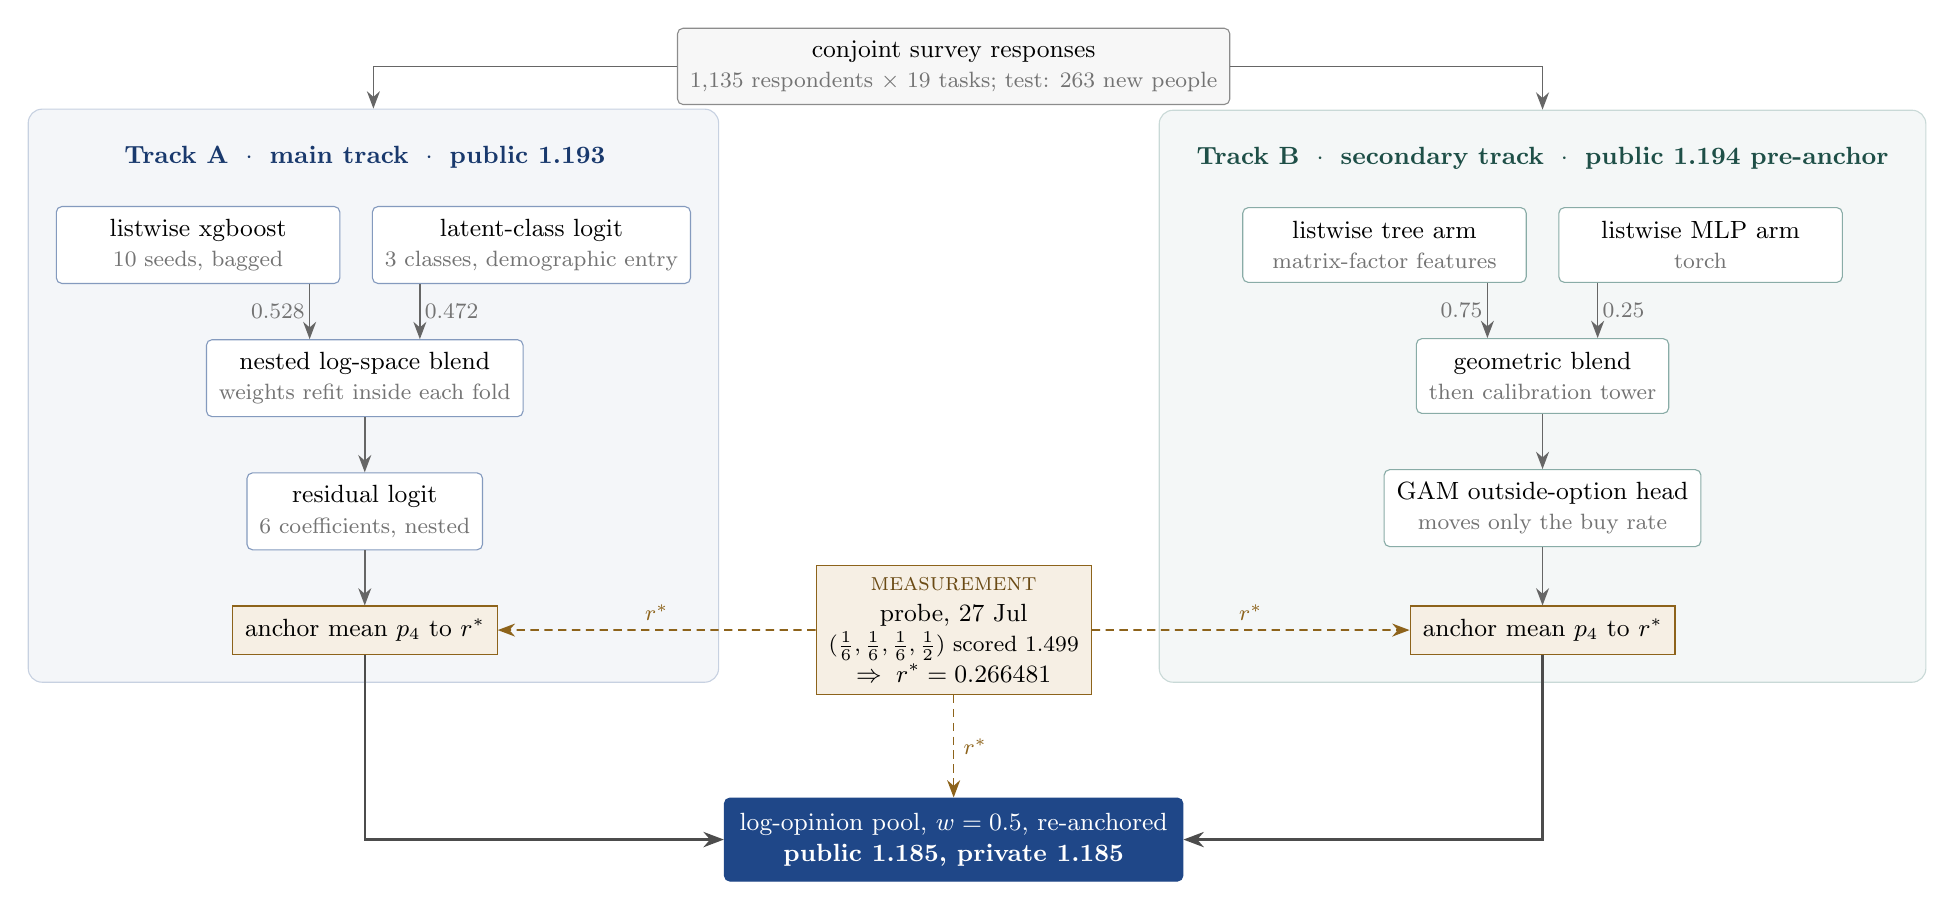
\begin{tikzpicture}[
  font=\small,
  box/.style={draw, rounded corners=2pt, align=center, inner sep=4.5pt, minimum height=9.5mm, fill=white},
  membA/.style={box, draw=acc!55},
  membB/.style={box, draw=accB!55},
  measbox/.style={draw=meas!80!black, fill=meas!12, align=center, inner sep=4.5pt},
  final/.style={draw=acc, fill=acc, text=white, rounded corners=2pt, align=center, inner sep=5.5pt},
  lane/.style={rounded corners=5pt, inner sep=3.5mm},
  arr/.style={-{Stealth[length=2.2mm]}, semithick, black!60},
  mainarr/.style={-{Stealth[length=2.6mm]}, thick, black!70},
  marr/.style={-{Stealth[length=2.2mm]}, semithick, densely dashed, meas!80!black},
  wlab/.style={font=\footnotesize, text=black!55, inner sep=1.5pt},
  node distance=7mm and 5mm]
\node[membA, minimum width=36mm] (xgb) {listwise xgboost\\{\footnotesize\color{black!55}10 seeds, bagged}};
\node[membA, minimum width=36mm, right=4mm of xgb] (lc) {latent-class logit\\{\footnotesize\color{black!55}3 classes, demographic entry}};
\node[membA, below=of $(xgb.south)!0.5!(lc.south)$] (blend) {nested log-space blend\\{\footnotesize\color{black!55}weights refit inside each fold}};
\node[membA, below=of blend] (rl) {residual logit\\{\footnotesize\color{black!55}6 coefficients, nested}};
\node[measbox, below=of rl] (ancA) {anchor mean $p_4$ to $r^{*}$};
\node[membB, minimum width=36mm, right=70mm of lc] (tree) {listwise tree arm\\{\footnotesize\color{black!55}matrix-factor features}};
\node[membB, minimum width=36mm, right=4mm of tree] (nn) {listwise MLP arm\\{\footnotesize\color{black!55}torch}};
\node[membB, below=of $(tree.south)!0.5!(nn.south)$] (gblend) {geometric blend\\{\footnotesize\color{black!55}then calibration tower}};
\node[membB, below=of gblend] (gam) {GAM outside-option head\\{\footnotesize\color{black!55}moves only the buy rate}};
\node[measbox] (ancB) at (gam |- ancA) {anchor mean $p_4$ to $r^{*}$};
\node[font=\small\bfseries, text=acc!80!black, anchor=south,
      above=3.5mm of $(xgb.north)!0.5!(lc.north)$] (labA) {Track A \(\;\cdot\;\) main track \(\;\cdot\;\) public 1.193};
\node[font=\small\bfseries, text=accB!75!black, anchor=south,
      above=3.5mm of $(tree.north)!0.5!(nn.north)$] (labB) {Track B \(\;\cdot\;\) secondary track \(\;\cdot\;\) public 1.194 pre-anchor};
\begin{scope}[on background layer]
\node[lane, fill=acc!5, draw=acc!25, fit=(labA)(xgb)(lc)(blend)(rl)(ancA)] (laneA) {};
\node[lane, fill=accB!5, draw=accB!25, fit=(labB)(tree)(nn)(gblend)(gam)(ancB)] (laneB) {};
\end{scope}
\node[box, draw=black!45, fill=black!3] at ($(labA.north)!0.5!(labB.north)+(0,9mm)$) (data)
  {conjoint survey responses\\{\footnotesize\color{black!55}1{,}135 respondents $\times$ 19 tasks; test: 263 new people}};
\node[measbox] at ($(ancA.east)!0.5!(ancB.west)$) (probe)
  {{\scshape\color{meas!60!black} measurement}\\probe, 27 Jul\\{\footnotesize $(\tfrac16,\tfrac16,\tfrac16,\tfrac12)$ scored 1.499}\\$\Rightarrow\; r^{*}=0.266481$};
\node[final, below=13mm of probe] (pool)
  {log-opinion pool, $w=0.5$, re-anchored\\\bfseries public 1.185, private 1.185};
\draw[arr] (data.west) -| (laneA.north);
\draw[arr] (data.east) -| (laneB.north);
\coordinate (bL) at ($(blend.north)+(-7mm,0)$);
\coordinate (bR) at ($(blend.north)+(7mm,0)$);
\coordinate (gL) at ($(gblend.north)+(-7mm,0)$);
\coordinate (gR) at ($(gblend.north)+(7mm,0)$);
\draw[arr] (bL |- xgb.south) -- node[wlab, left]{0.528} (bL);
\draw[arr] (bR |- lc.south) -- node[wlab, right]{0.472} (bR);
\draw[arr] (blend) -- (rl);
\draw[arr] (rl) -- (ancA);
\draw[arr] (gL |- tree.south) -- node[wlab, left]{0.75} (gL);
\draw[arr] (gR |- nn.south) -- node[wlab, right]{0.25} (gR);
\draw[arr] (gblend) -- (gam);
\draw[arr] (gam) -- (ancB);
\draw[mainarr] (ancA.south) |- (pool.west);
\draw[mainarr] (ancB.south) |- (pool.east);
\draw[marr] (probe.west) -- node[above, font=\footnotesize]{$r^{*}$} (ancA.east);
\draw[marr] (probe.east) -- node[above, font=\footnotesize]{$r^{*}$} (ancB.west);
\draw[marr] (probe.south) -- node[right, font=\footnotesize]{$r^{*}$} (pool.north);
\end{tikzpicture}

% ---------------------------------------------------------------- figure 2
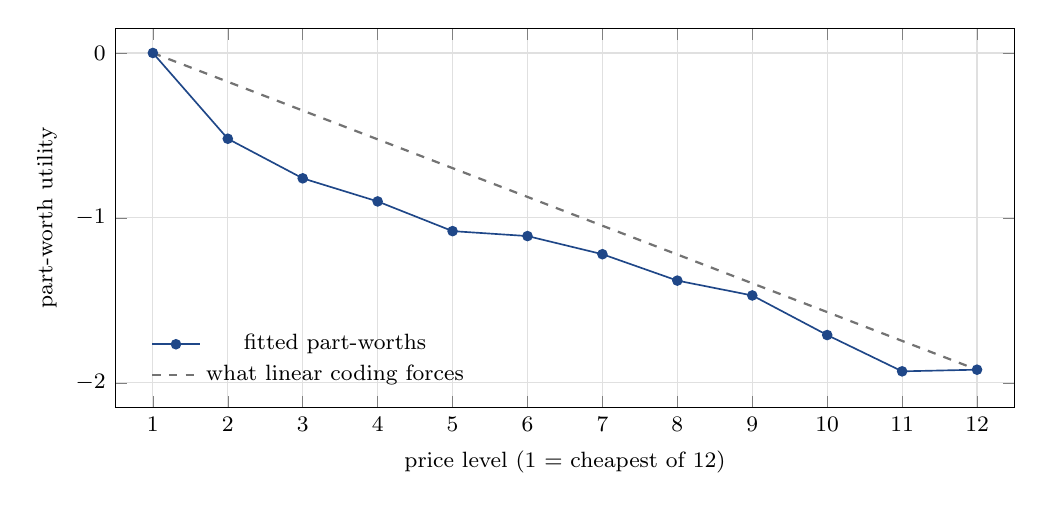
\begin{tikzpicture}
\begin{axis}[
  width=13cm, height=6.4cm,
  xlabel={price level (1 = cheapest of 12)}, ylabel={part-worth utility},
  xmin=0.5, xmax=12.5, ymin=-2.15, ymax=0.15,
  xtick={1,...,12}, tick label style={font=\footnotesize},
  label style={font=\footnotesize},
  grid=major, grid style={black!12},
  legend style={font=\footnotesize, at={(0.03,0.03)}, anchor=south west, draw=none, fill=none}]
\addplot[color=acc, mark=*, mark size=1.6pt, semithick] coordinates
{(1,0) (2,-0.52) (3,-0.76) (4,-0.90) (5,-1.08) (6,-1.11) (7,-1.22) (8,-1.38) (9,-1.47) (10,-1.71) (11,-1.93) (12,-1.92)};
\addlegendentry{fitted part-worths}
\addplot[color=black!55, dashed, thick] coordinates {(1,0) (12,-1.92)};
\addlegendentry{what linear coding forces}
\end{axis}
\end{tikzpicture}

% ---------------------------------------------------------------- figure 3
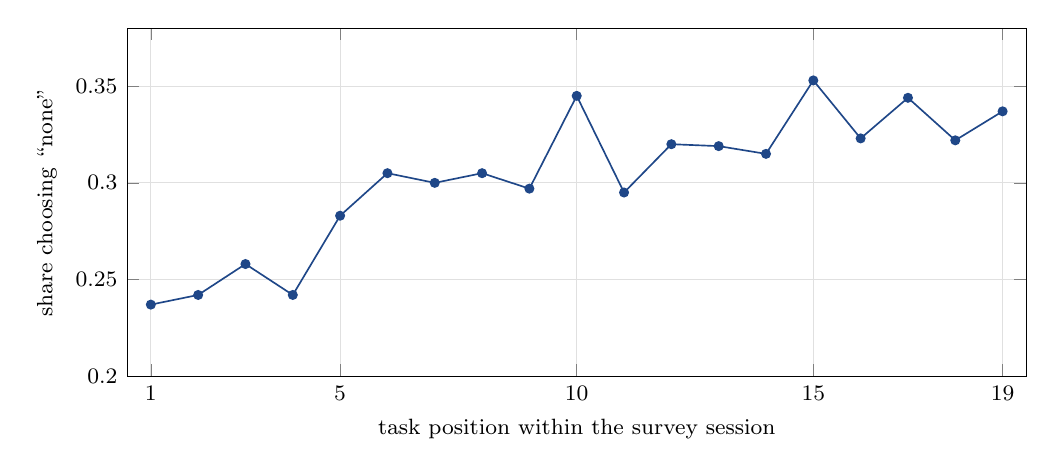
\begin{tikzpicture}
\begin{axis}[
  width=13cm, height=6.0cm,
  xlabel={task position within the survey session}, ylabel={share choosing ``none''},
  xmin=0.5, xmax=19.5, ymin=0.20, ymax=0.38,
  xtick={1,5,10,15,19}, ytick={0.20,0.25,0.30,0.35},
  tick label style={font=\footnotesize},
  label style={font=\footnotesize},
  grid=major, grid style={black!12}]
\addplot[color=acc, mark=*, mark size=1.5pt, semithick] coordinates
{(1,0.237) (2,0.242) (3,0.258) (4,0.242) (5,0.283) (6,0.305) (7,0.300) (8,0.305)
 (9,0.297) (10,0.345) (11,0.295) (12,0.320) (13,0.319) (14,0.315) (15,0.353)
 (16,0.323) (17,0.344) (18,0.322) (19,0.337)};
\end{axis}
\end{tikzpicture}

\end{document}
